




\chapter{Konzept}
Im Folgenden wird die Anwendung der in Kapitel 2 erläuterten Grundkonzepte beschrieben. Dabei wird zunächst auf den Entwurf der Software eingegangen, anschließend auf die prototypische Implementierung.\\

\section{Ausgangssituation}
In der Ausgangssituation wird der aktuelle Stand der Forschung im Bereich RFU-Client in Verbindung mit einem \ac{opcua}-Server und die Verbindung mit dem UAExpert untersucht. Es wird auch untersucht, was bisher mit Node \ac{opcua} erforscht wurde und welche \ac{opcua}-Clients bisher für den RFU verfügbar sind.

%aktueller Stand der Forschung
%welche verbindungen gibt es mit dem UAExpert? 
%Was wurde bisher mit node opcua gemacht?
%Welche Client gibt es bisher?
\subsection{Schnittstellen zum Server}
Auf dem RFU läuft ein \ac{opcua}-Server, der auf verschiedene Arten abgefragt wird. Einerseits gibt es verschiedene Clients, die in den Programmiersprachen Python, C\# oder C implementiert sind und alle mit dem Stack ihrer jeweiligen Programmiersprache arbeiten. Andererseits ist es auch möglich, den \ac{opcua}-Server mithilfe von UAExpert abzufragen und Daten zu empfangen.\\

Die Verbindung zum RFU wird über ein LAN-Kabel und einen USB-Internet-Adapter hergestellt. Der Internet-Adapter wird verwendet, da er frei konfiguriert werden kann. Die IP-Adresse des RFUs und des Internet-Adapters müssen im gleichen Subnetz liegen. Zunächst wird die IP-Adresse des RFUs konfiguriert. Diese kann über Sopas ET eingestellt werden. Danach wird die IP-Adresse des USB-Internet-Adapters konfiguriert.\\

Im UAExpert wird ein Server hinzugefügt. Unter \frqq Custom Discovery \flqq wird auf den \ac{opcua}-Server des RFUs über dessen zuvor konfigurierte IP-Adresse zugegriffen. In diesem Fall wird diese IP-Adresse genutzt: \frqq opc.tcp://192.168.136.2:4840 \flqq \\

\subsection{Die Struktur des Sensors}

Der UA-Experte ist in der Lage, die Objekte des Servers und die dazugehörigen Methoden mit Variablen des Servers auszulesen und grafisch darzustellen. Die Struktur des Sick RFU besteht aus vielen Knoten, von denen jeder aus verschiedenen Elementen besteht. Die Struktur des Sick RFU wird im Address Space Window dargestellt.\\

\begin{figure}[htp]
    \centering
    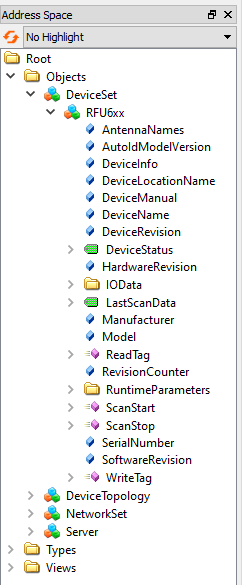
\includegraphics[width=(\textwidth/3)]{Bild/Address_Space.PNG}
    \caption{Address Space Window}
    \label{fig:Address Space Window}
\end{figure}

In der Abbildung \ref{fig:Address Space Window} wird die Struktur des Sensors mit seinen verschiedenen Elementen dargestellt, wobei jedes Element über einen eigenen Knoten verfügt. 
\frqq DeviceSet\flqq, \frqq RFU6xx\flqq, \frqq DeviceTopology\flqq, \frqq Networkset\flqq und \frqq Server\flqq sind Objekte, während die restlichen Elemente Methoden und Variablen darstellen. 
Im Rahmen dieses Projekts werden ausschließlich die in Lila markierten Methoden sowie der Knoten RFU6xx \frqq LastScanData\flqq benötigt. 
\frqq ReadTag\flqq, \frqq StartScan\flqq, \frqq WriteTag\flqq, \frqq StopScan\flqq und \frqq LastScanData\flqq sind die Methoden die in dem Node.js Client implementiert werden.

\subsection{Herstellung einer Verbindung}
Der \ac{opcua}-Client wird durch Node \ac{opcua} Bibliothek, die es ermöglicht, \ac{opcua}-Verbindungen aufzubauen. Die Bibliotheken erfordern die Angabe von entsprechenden Verbindungsdetails. Um den Client mit dem Server zu verbinden, wird die Bibliothek die Verbindungsdetails verwenden, die bei der Erstellung des Clients angegeben sind.
\begin{lstlisting}[style=JavaScript, caption={Node OPCUAClient Create}]
const options = {
    applicationName: "MyClient",
    connectionStrategy: connectionStrategy,
    securityMode: MessageSecurityMode.None,
    securityPolicy: SecurityPolicy.None,
    endpointMustExist: false,
};
const client = OPCUAClient.create(options);
const endpointUrl = "opc.tcp://192.168.136.2:4840";
async function main() {
    await client.connect(endpointUrl);
    console.log("connected !");
    const session = await client.createSession();
    console.log("session created !");
    await session.close();
    await client.disconnect();
    console.log("done !");
}
\end{lstlisting}

Der verwendete Port hängt von der Konfiguration des Servers und der verwendeten Verbindungsmethode ab. Standardmäßig wird in der Regel Port 4840 für \ac{opcua}-Verbindungen verwendet.

Eine Session ist eine Verbindung zwischen dem \ac{opcua}-Client und dem Server. Um eine Sitzung zu erstellen, muss der Client zunächst eine Verbindung zum Server herstellen und dann eine Anforderung für eine Sitzung senden. Die Node \ac{opcua}-Bibliotheken enthalten Funktionen zum Erstellen von Sitzungen.

Die Sitzung wird geschlossen, indem der \ac{opcua}-Client eine Anforderung zum Beenden der Sitzung sendet. Die Node \ac{opcua}-Bibliotheken verfügen über Funktionen zum Schließen von Sitzungen.

\subsection{RFU6xx Clients in anderen Programmiersprachen}

Es gibt bisher drei \ac{opcua}-RFU-Clients in verschiedenen Programmiersprachen. Die \ac{opcua}-RFU-Clients aus dem Hause Sick sind in den Programmiersprachen C\#, C und Python programmiert.\\

Die verschiedenen Clients greifen weitestgehend auf die gleichen Funktionen des \ac{opcua}-Servers des RFUs zu. \frqq ReadTag\flqq, \frqq StartScan\flqq, \frqq WriteTag\flqq, \frqq StopScan\flqq und \frqq LastScanData\flqq sind die Methoden, über die alle Clients verfügen.\\

Die Clients in den Programmiersprachen Python und C\# greifen auf die Funktionen des RFUs über eine Klasse zu, da sie es ermöglichen, objektorientiert zu programmieren. So können die Clients einfacher ausgelagert und spezifizierter verwendet werden. Der RFU-Client in der Programmiersprache C ist imperativ geschrieben.\\

Die RFU-Clients nutzen die Stacks ihrer Programmiersprache. Ein \ac{opcua}-Stack umfasst typischerweise verschiedene Module, einschließlich Transportebenen, Kodierungs- und Dekodierungsmodulen sowie Sicherheitsmodulen. Diese Module arbeiten zusammen, um eine vollständige Implementierung des \ac{opcua}-Protokolls bereitzustellen.\\

\ac{opcua}-Stacks können von Softwareentwicklern verwendet werden, um \ac{opcua}-fähige Anwendungen zu erstellen. Durch die Verwendung eines \ac{opcua}-Stacks können sich Entwickler auf ihre Anwendungslogik konzentrieren, ohne die Low-Level-Details des Protokolls implementieren zu müssen. Es gibt mehrere kommerzielle und Open-Source-\ac{opcua}-Stacks, die jeweils ihre eigenen Stärken und Schwächen haben.\\




\section{Softwareentwurf}


TypeScript ermöglicht sowohl imperatives als auch objektorientiertes Programmieren. Die Wahl hängt von der spezifischen Anforderung und Präferenz des Entwicklers ab.\\

Imperative Programmierung ist eine Programmiermethode, bei der das Programm als eine Folge von Anweisungen geschrieben wird, die in der Reihenfolge ausgeführt werden, in der sie geschrieben wurden. Sie ist nützlich, wenn Sie eine schnelle Lösung für ein bestimmtes Problem benötigen oder wenn Sie ein kleines Skript schreiben.\\

Objektorientierte Programmierung hingegen ist eine Programmiermethode, bei der das Programm als Zusammenstellung von Objekten und deren Interaktion geschrieben wird. Sie ist nützlich, wenn Sie eine komplexe Anwendung mit vielen Modulen und Komponenten schreiben. Mit objektorientierter Programmierung können Sie Ihre Codebasis besser strukturieren und wiederverwendbaren Code erstellen.\\

Für den spezifischen Einsatz des RFU-Clients wird er objektorientiert programmiert, damit er ausgelagert werden kann.\\

\subsection{Anforderungen}


Der RFU-Client soll leicht verständlich und leserlich sein.\\

Zunächst sollen Kommentare verwendet werden, um den Code zu dokumentieren und den Zweck der verschiedenen Abschnitte zu erklären. Dies kann dazu beitragen, dass der Code leichter zu verstehen ist, insbesondere wenn er komplexer wird.\\

Eine klare und konsistente Benennung von Variablen, Funktionen und Klassen, um den Code leichter lesbar und verständlich zu machen. Namen die den Zweck und die Funktion der Elemente klar ausdrücken.\\

Whitespace soll auch verwendet werden, um den Code leichter lesbar zu gestalten. Den Code so anordnen, dass er in Abschnitte oder Blöcke unterteilt ist, und Leerzeichen verwenden, um die verschiedenen Teile des Codes voneinander abzugrenzen.\\

Übermäßige Verschachtelung vermeiden, die den Code schwer lesbar machen kann. Stattdessen Funktionen oder Klassen, um den Code in kleinere Teile zu zerlegen, die zu verstehen sind.\\

\subsection{Systemumgebung}
Zudem wird in einer VM Programmiert. Programmiert wird in Nodepad++ und in vs code. Versioniert wird mit github.

\subsection{Programmdesgin}


\section{Vorgehensweise}
Wie wurde vorgegangen?
Woher wurden informationen gezogen?
Welche Beesonderheiten hatte TypeScript?


Der Python-Client, der als Vorlage dient, zeigt eine mögliche Implementierung eines Clients für ein Remote Field Unit 6xx (RFU6xx)-Gerät, das mit dem \ac{opcua}-Protokoll kommuniziert. Der Client ist in der Programmiersprache Python geschrieben und nutzt die Bibliothek "opcua" für die Kommunikation mit dem Gerät über das \ac{opcua}-Protokoll.\\

Die im Python-Client verwendeten Funktionen und Klassen können als Referenz für die Implementierung eines ähnlichen Clients in einer anderen Programmiersprache verwendet werden. Dabei können die verwendeten Konzepte wie asynchrone Programmierung, Verwendung von Namespace-Indizes, Anwendung von Strukturierungsmustern wie Funktionen und Klassen sowie die Verwendung von ExtensionObjects und Nodes für die Interaktion mit dem Gerät nützlich sein.\\

Es ist jedoch zu beachten, dass die tatsächliche Implementierung eines \ac{opcua}-Clients je nach Sprache und Bibliothek, die verwendet wird, unterschiedlich sein kann. Daher sollte der Python-Client als Beispiel und nicht als exakte Vorlage verstanden werden.\\






